\chapter{Experimental results \statusfirstdraft}
\label{chap:results}

In this chapter we quantitatively and qualitatively analyse the performance of the automatic cell detector and tracker. Although some evaluation of the performance of the detection method is performed by the original authors in \cite{arteta12} it is useful to see how the method performs on the studied datasets in order to understand how much of the tracking accuracy is lost due to cells missed by the detection module. First, in \cref{sec:results_detector} we evaluate the performance and computation time of the cell detector and in \cref{sec:results_tracker} those of the cell tracker. Finally, in \cref{sec:results_limitations}, we explore the limitations of the methods and in \cref{sec:results_summary} summarize the results.

\section{Cell detector \statusfirstdraft}
	\label{sec:results_detector}
	
	In this section we evaluate the performance of the automatic cell detection module. First, we introduce the performance metrics used to evaluate the accuracy of the cell detector. Then we present detection accuracy results. To evaluate the accuracy and generalizability of the detection module we perform two sets of experiments. First, we train the cell detector on a number of frames from each individual dataset, and measure the accuracy on the same dataset. Second, we train the detector on combinations of datasets in order to judge the performance degradation due to the learning on the more types of cells. Because of the varying size of the cells in the datasets, and the varying brightness of the cells, we expect that such a trained detector will perform poorer than when trained and tested on individual datasets, sometimes mistakenly detecting small artefacts in the background as cells. Finally, we compute the average detection time per frame for each dataset.
	
	The aim of this research was to develop an automatic cell detection and tracking pipeline that would require as little manual work as possible. This implies that a balance between accuracy and amount of manual work had to be established. There is also an direct relationship between accuracy and computation time. In order to reduce the amount of manual work we aimed to configure the cell detection module such that it would perform well on all the tested datasets without any manual adjustments of parameters. The consequences of this decision are twofold:
	
	\begin{enumerate}
		\item The features computed on the candidate cell regions are the same for all datasets and have been presented in \cref{sec:detector_feature}. Although some datasets could be analysed faster or more accurately with a different subset of features, using the same features for all dataset eliminates the complicated feature selection process for the user and makes the system generalizable to a large number of different cell types.
		
		\item The parameters of the MSER detector should be adequately set to perform well on all datasets. This means that the MSER detector should be able to detect cells of varying size and contrast in the different datasets. The consequence of this limitation for datasets with large cells and some background noise is that a potentially much larger number of candidate regions will be detected than necessary. Since each candidate region has to be evaluated this results in an increased computation time.
	\end{enumerate}
	
	We were able to identify features that compute in an acceptable time for all these datasets (see \cref{sec:detector_feature}). However, it should be noted that in the case of testing the detector on very large datasets with thousands of frames, some adjustments of the parameters could result in a significant reduction in computation time and increased accuracy.
	
	\subsection{Performance metrics \statusfirstdraft}
	
	We measure the performance of the cell detector in terms of precision and recall. The metrics are defined in terms of:
	
	\begin{description}
		\item[True Positive instances] (TP) are candidate cell regions that are manually annotated as cells and the detector successfully classified as cells.
		\item[False Positive instances] (FP) are candidate cell regions that are not manually annotated as cells, but the detector incorrectly classified them as cells.
		\item[False Negative instances] (FN) are candidate cell regions that are manually annotated as cells, but the detector incorrectly classified.
	\end{description}
	
	We then define precision as:
	
	\[
		\text{PRE} = \frac{\text{TP}}{\text{TP}+\text{FP}}\text{,}
	\]
	
	\noindent and recall (also known as sensitivity) as:
	
	\[
		\text{REC} = \frac{\text{TP}}{\text{TP} + \text{FN}}\ \text{.}
	\]
	
	\subsection{Detection accuracy \statusfirstdraft}
			
		As mentioned previously, we performed two different experiments to measure the performance of the cell detection module. The first experiment consisted of training and testing of the algorithm on the same dataset. The training set was 70\% and the testing set 30\% of the entire dataset. The training and testing datasets were created from images in randomized order from the entire dataset. This allowed us to measure, for each dataset, the maximum precision and recall values we could expect from the algorithm. In the second experiment the training was performed on combined datasets. The goal of this experiment was to observe how well the algorithm is able to generalize, and still return acceptable results.
		
		\subsubsection{Training and testing on individual datasets}
		
		The training was performed on 70\% of the manually dot-annotated images from each dataset, and tested on the remaining 30\%. \Cref{tab:results_detector_individual} displays the computed precision and recall values.
		
		
		\begin{table}[h]
			\centering
			\begin{tabular}{rrr}
				Dataset & Precision & Recall \\
				\hline
				      A &      25.0 &   22.5 \\
				      B &      90.1 &   89.1 \\
				      C &      76.5 &   84.2 \\
				      D &      86.1 &   85.3 \\
				      E &      93.4 &   78.6
			\end{tabular} 
			\caption{Precision and recall values for the cell detector trained on each dataset individually.}
			\label{tab:results_detector_individual}
		\end{table}
		
		The detector tested on datasets B to E achieved precision and recall values above 75. A manual comparison of the annotation confirms that the results are good, with few bad detections. Most of the differences in detection were caused by minor inconsistencies in annotations. The importance of consistent annotations was stressed in \cref{sec:data_manual_annotation}.
		
		Dataset A is an outlier with extremely low precision and recall values. This is likely caused by the specific characteristics of this image sequence, which we described in \cref{subsec:datasetA}. Briefly, between frame 17 and 18 there is an abrupt change of image clarity. The background from the threshold frame onwards have a texture that is very similar to that of the cells in the first 17 frames. This means that the negative candidate regions from frame 18 and onward clash with the positive candidate regions from the previous frames. The result is that the detector is unable to learn to discriminate cells from background.
		
		These results show us the detector can correctly detect most of the (annotated) cells. Further manual reviews of the annotations would likely improve the performance, but this is not done here as it should have been tested on a separate validation dataset. Additionally, it is unlikely that future users of this detection method will always have perfect annotations available. In the next experiment, we will measured the performance of the detector when trained on a composite dataset. This will tell us whether it would be possible to learn a single, general detector and use it to test on a new, possibly unforeseen datasets.

		\Cref{fig:results_detector_sequences_1,fig:results_detector_sequences_2,fig:results_detector_sequences_3,fig:results_detector_sequences_4,fig:results_detector_sequences_5} in appendix \ref{app:appendix_detectionresults} display a temporal view of the detected results in each datasets. The vertical axis represents the consecutive frame number of the image sequence. The figures show that ``cell tracks'' are discernible, even if the number of outliers is significant. The detectors used to detect the cells on the entire dataset were trained on all the annotated frames.

		\subsubsection{Training on combined datasets}
		
		In this second experiment we were interested in measuring how well the algorithm is able to generalize when it is trained on a larger, combined dataset. For this purpose, several of the datasets were grouped, and the detector was trained to recognize cells of all types. The detector was trained on a random 70\% of all annotated images in the combined dataset. It was then tested on a random 30\% of annotated frames from each individual dataset separately. This means that sometimes the same frames could be used for training and testing. However, we also run combinations of datasets where one dataset is left out of training at each time. Testing on that dataset should then reveal if the algorithm generalizes well.
		
		\Cref{tab:results_detector_combined} summarizes the precision and recall values for all tested combined datasets. The column denoted $\gamma$ contains testing performance as tested on 30\% of the combined dataset. The values shown in bold correspond to the performance of testing on the dataset that was left out from the combined training dataset. The row denoted ``Individual'' indicates the results when the datasets where trained and tested individually (these are the same results as in \cref{tab:results_detector_individual}). The values shown in red indicate a decrease in precision/recall by at least 1 point compared to the results when trained and tested on individual datasets. Similarly, blue colour indicates an increase in precision/recall compared to the results on the row denoted ``Individual''.
		
		\begin{table}[h]
			\centering
			\begin{tabular}{c|*{6}{c}|*{6}{c}}
				\multicolumn{1}{c}{Dataset} & \multicolumn{6}{|c|}{Precision}                                              &                          \multicolumn{6}{c}{Recall}                          \\
				                            & $\gamma$ &     A      &     B      &     C      &     D      &       E       & $\gamma$ &     A      &       B       &     C      &     D      &     E      \\
				        Individual          &          &    25.0    &    90.1    &    76.5    &    86.1    &     93.4      &          &    22.5    &     89.1      &    84.2    &    85.3    &    78.6    \\
			\hline
				           ABCDE            &   74.5   & \up{49.2}  & \dn{76.0}  & \up{85.2}  & \dn{69.2}  &   \up{94.5}   &   79.9   & \up{58.3}  &   \up{90.8}   & \dn{57.1}  & \up{98.9}  & \up{79.7}  \\
			\hline
				          ABCD\_            &   69.7   & \up{49.2}  & \dn{77.0}  & \up{85.8}  & \dn{69.9}  & \textbf{93.4} &   80.0   & \up{58.3}  &     90.3      & \dn{58.7}  & \up{98.4}  & \upd{80.7} \\
				          ABC\_E            &   72.8   & \up{45.9}  & \dn{75.0}  & \up{82.6}  & \dnd{41.1} &   \dn{87.2}   &   83.2   & \up{65.0}  &   \up{96.4}   & \dn{73.6}  & \upd{99.4} & \up{89.8}  \\
				          AB\_DE            &   75.5   & \up{47.5}  & \dn{75.8}  & \upd{85.7} & \dn{73.1}  &   \up{96.5}   &   73.1   & \up{50.8}  &     88.9      & \dnd{46.1} & \up{97.1}  & \dn{68.3}  \\
				          A\_CDE            &   75.9   & \up{41.3}  & \dnd{63.1} & \up{85.5}  & \dn{71.2}  &   \up{94.6}   &   70.4   & \up{58.3}  & \textbf{89.2} & \dn{57.0}  & \up{99.0}  & \up{80.2}  \\
				          \_BCDE            &   86.3   & \upd{49.2} & \dn{76.4}  & \up{85.9}  & \dn{71.8}  &   \up{94.4}   &   76.4   & \upd{58.3} &     89.5      & \dn{56.0}  & \up{97.4}  & \dn{75.7}  \\
			\hline
				          \_BCD\_           &   82.8   & \upd{52.5} & \dn{78.0}  & \up{87.5}  & \dn{72.7}  &  \upd{95.2}   &   74.5   & \upd{55.8} &     89.5      & \dn{54.7}  & \up{97.4}  & \dnd{74.0} \\
				          \_B\_DE           &   85.9   & \upd{42.5} & \dn{80.3}  & \upd{84.8} & \dn{72.1}  &   \up{97.7}   &   82.6   & \upd{45.8} &   \up{91.2}   & \dnd{44.8} & \up{97.4}  &  \dn{66.3}
			\end{tabular} 
			\caption{Precision and recall values for the cell detector trained on combined datasets. Values typed in bold indicate the testing datasets that were not included in the combined training dataset. Red/blue colour indicates a decrease/increase in performance compared to training and testing on each individual dataset by at least 1 precision/recall point.}
			\label{tab:results_detector_combined}
		\end{table}
		
		The values in the table show us some significant insights. First of all, the recall values increased for most datasets when detecting cells using a detector trained with almost any combination of data. Using more data thus improves the recall. This means that in general the algorithm will detect a larger number of true positive instances, but also some false negatives. However, given the high recall value we can expect the number of false negatives to remain relatively small. For the tracking module it is easy to discard short, isolated detections. The high recall values indicate that we will likely detect most of the real cell trajectories.
		
		Second, we notice that while most recall increase, precision tends to decrease in some datasets. This means that the number of false positives increased. As said beforehand, the cell tracking module can deal effectively with short, isolated false positives. However, if the number of false positives increases too much, the tracking module might detect cell trajectories where there are none (or correspond to background noise). However, given that in most examples the precision values did not fall below 70 we should still expect to achieve good tracking results.
		
		The results on Dataset C went against these observations. Its recall values decreased significantly whenever a combined dataset was used to train the detector. This dataset contains many motion artefacts, and high variance of intensities of the cells, some of which smoothly blend into the background. This makes it very difficult to consistently annotate. It is possible that the inconsistencies in annotation make it perform in such a way when combined with other datasets.
		
		Another interesting observation is that the precision and recall values for dataset A improved significantly compared to training the detector only on dataset A. We have previously presented some possible reasons for its poor performance when trained individually. The increased performance when using a cell detector trained on other datasets (even excluding dataset A itself) can be attributed to two things. First, the detector learns to detect a wider range of types of cells. Second, dataset A contains much fewer annotated cells than the other datasets (about five times less). It is possible that a detector trained on only dataset A overfits the annotations, and cannot generalize to detect cells in other frames. 
		
		The performance on dataset E remained almost constant, with very few exceptions (e.g. smaller recall value when the detector was trained on combined dataset containing datasets A, B, D and E).

		In this section we aimed to understand whether a detector trained on a single, combined dataset could be used to detect cells in new, previously unseen images. The results have shown that a general detector will not perform well on \textit{all} new unseen datasets. For example, we have measured a significant drop in precision values when testing on unseen datasets B and D, and a significant drop in recall values when testing on dataset C. However, in some cases training on a combined detector either improved the performance or reduced it insignificantly (such as in datasets A and E). What this tells us is that when presented with a new dataset it is worth trying to use a pre-trained detector and review its results. In some cases this could give as acceptable results, and manual annotation of the new dataset might be unnecessary.
		
		It is worth keeping in mind that all five datasets analysed in this thesis show distinct characteristics (both in cell type and image clarity). In practice, datasets will often be similar and it might be sufficient to annotated a single dataset to train a detector that can be used on other similar samples.
	
	\subsection{Computations time \statusfirstdraft}
	
		In order to positionally track cells in image sequence the computation time of extracting the cell position from each frame is just as important as the accurate identification of cells. \Cref{tab:results_detector_speed} displays the average detection times per frame for each dataset. We also measured the average detection time per annotated cell in each dataset and the average ratio between the number of all candidate regions that were detected with the MSER detector and the number of annotated cells in each frame.
		
		The detection was performed on a PC with an Intel(R) Core(TM) i7-2600 CPU with a clock frequency of 3.40GHz and 8GB RAM. The MATLAB version used to measure the detection speed was 8.1.0.604 (R2013a) running in Ubuntu Linux 13.04 x64. Althought the detector can be easily configured to use several workers to process the image sequences in parallel, the measurements were performed using a single worker, i.e. all images was processed sequentially.
		
		\begin{table}[h]
			\centering
			\begin{tabular}{rrrr}
				Dataset & Time per frame  $\left[ s \right]$ & Time per annotated cell  $\left[ s \right]$ & Candidate-Annotation ratio \\
			\hline
				      A &                             0.7458 &                                      0.4733 &                       36:1 \\
				      B &                             1.4466 &                                      0.1801 &                       18:1 \\
				      C &                             1.2730 &                                      0.1422 &                       11:1 \\
				      D &                             1.3607 &                                      0.9378 &                       21:1 \\
				      E &                             0.6273 &                                      0.2589 &                       13:1
			\end{tabular} 
			\caption{Average computation times per frame and annotated cell.}
			\label{tab:results_detector_speed}
		\end{table}

		The results show that we were able to optimize the cell detector to a point where it's speed is no longer an issue for many use cases. As a reminder, the original paper by Arteta \emph{et. al.} \cite{arteta12} reports detection speeds of 30 seconds per 400-by-400 pixels image on an i7 CPU. Most of the computation time is spend by the MSER detector and the feature computation.
		
		The measurements show that the detection speed is dependent primarily on the number of cells in each frame. Datasets B, C, and D contain 5 to 10 times more cells per frame than dataset A. Dataset E also contains 5 times more cells than dataset A, but it's computation time per frame was lower. This could be attributed to the smaller fraction of candidate regions that had to evaluated. In contrast, in dataset A which contains larger cells than the other datasets many more candidate cells were evaluated relative to the number of annotated cells. It is likely that, since the MSER detector was configured equally for all datasets, the MSER detector identified a larger number of small noise artefacts as cell candidates.
		
\section{Cell tracker \statusfirstdraft}
	\label{sec:results_tracker}
	
	After obtaining the cell detection results we must determine the number of trajectories and which detection results belong to which trajectory. In the analysis of the performance of the tracking system we assume that the detection results are already available. The cell detector had been trained on the annotated images from each dataset, and the cells have been identified on the entire image sequences. Similarly to the experiments run on the cell detection module, we also run two sets of experiments for the cell tracker. First, we measure the performance of the cell tracker after being trained and tested on each dataset individually. In the second experiment we train the cell tracking module on combined datasets and evaluate its performance on previously unseen trajectories.
	
	The aim of this research was to develop an automatic cell detection and tracking pipeline that would require as little manual work as possible. However, there are a few cases when an automated algorithm might not perform with the desired accuracy, for example when testing on a new dataset and reusing a tracker trained on a different dataset. For this reason four intuitive parameters can be adjusted to modify the tracking results. We discussed the benefits of this configuration in \cref{sec:tracking_scalingparameters}.
	
	Further, in order to evaluate the cell tracking module, we are interested in two things. First, how well do the generated trajectories fit the ground truth annotations. This measure is dependent on the effectiveness of the cell tracker module as well as the cell detection module. This is a measure of how well the automatic tracking pipeline works. However, if the cell detection module misses too many cells, it might be impossible for the tracking module to compensate for the errors. Therefore, we are also interested in how well the developed tracking module works independently of the cell detection module. This can give us an idea of how much of the performance is lost in the tracking module, given perfect detection results. For this reason the following scenarios will be evaluated:
	
	\begin{enumerate}
	\item Performance relative to the Ground Truth annotations (GT-P). This is a measure of how well the combination of the cell detector and tracker perform together.
	\item Performance relative to \textit{Detected Ground Truth annotations} (DGP-P). \textit{Detected ground truth annotations} are obtained by automatically mapping the ground truth annotations to the cell detection results. For example, a ground truth annotated trajectory is mapped to detection results by finding for each annotated cell observation of the trajectory a detection result that is less than a certain number of pixels away (e.g. 10 pixels). This measure compares the \textit{detected ground truth annotations} to the generated trajectories and gives a measure that is less dependent on the performance of the cell detection module.
	\item Comparison of Ground Truth annotation and \textit{Detected Ground Truth annotations} (GT-DGT-P). This measure does not measure the quality of the generated trajectories, but measures the performance lost due to errors in the cell detection module. 
	\end{enumerate}
	
	These performance evaluations measure the performance of the longest ground truth trajectories. Annotating all the trajectories in the full datasets would require weeks of manual work and review to assert the correctness of the annotations. For this reason testing is limited to a certain number of long fully annotated trajectories which have been manually identified and annotated. The counts of the annotated trajectories together with their length is available in \cref{tab:results_counttrajectories}.
	
	\begin{table}[h]
		\centering
		\begin{tabular}{rcr}
			  Dataset & Annotated trajectories &                              Length (number of frames) of annotated trajectories \\
		\hline
			Dataset A &           2            &                                                                         49    25 \\
			Dataset B &           14           & 66    65    60    51    46    41    37    29    26    19    18    15    14    10 \\
			Dataset C &           8            &                                          118   118    97    83    81    74    71 \\
			Dataset D &           6            &                                                      267   164   116   112   107 \\
			Dataset E &           8            &                                          117   110   105    93    73    51    37
		\end{tabular} 
		\caption{Count and length of manually annotated trajectories in each dataset.}
		\label{tab:results_counttrajectories}
	\end{table}

	All the measurements of the cell tracker performance have been obtained by cross validation. Because the number of annotated trajectories is relatively small, we have used leave-one-out cross validation. This involves repeatedly partitioning the set of annotated trajectories into two subsets, training the tracker on the training subset, and measuring its performance on the testing subset. As the name suggests, in each round we train the tracker on all but one annotated trajectory, using the left-out trajectory for measuring the performance. This is repeated for each annotated trajectory and the results are averaged over all the rounds.

	\subsection{Performance metrics \statusfirstdraft}
	
	To quantify the performance of the cell tracking module we use two metrics originating from radar tracking literature \cite{blackman99}, recently used in other works \cite{bise11global, huh13, eom07}: \textit{target effectiveness} and \textit{track purity}.
	
	Let us call a \textit{target} a true cell trajectory as provided by manual ground truth annotations and \textit{track} the generated trajectory by the cell tracker module. Then, for a target and track pair, target effectiveness can be defined as:
	
	\[
		\text{Target Effectivenes} = \frac{\text{100 $\times$ Number of frames where the target is correctly followed by the track}}{\text{Total number of frames of the target}}\text{.}
	\]
	
	Note that the multiplication by 100 is simply to represent the output from 0 to 100 instead of 0 to 1. 	Target effectiveness therefore tells us how effectively a target if followed by a track. For each target we find the track that follows it correctly for the longest number of frames. The measure penalizes tracks that are initialized late or terminated early relative to the target. However, it does not penalize tracks for being initiated early, or terminated late. Therefore, we need an additional measure, track purity, which does just that. In the case of track purity the roles of track and target are inverted. It measures how well the target follows a track, and is defined as:
	
	\[
		\text{Track Purity} = \frac{\text{100 $\times$ Number of frames where the track is correctly followed by the target}}{\text{Total number of frames of the track}}\text{.}
	\]
	
	This measure will penalize early initiated or late terminated tracks. It is similar to precision in that it penalizes false detections. We measure it by assigning to each track the target that follows it for the longest number of frames. 
	
	\subsection{Tracking accuracy \statusfirstdraft}
	
	
		As mentioned previously, we performed two different experiments to measure the performance of the cell tracking module. The first experiment consisted of training and testing of the algorithm on the same dataset. The performance evaluation was performed by leave-one-out cross validation where we repeatedly train the model on $n-1$ annotated trajectories and test it on the trajectory that was left out. This first experiment allowed us to measure, for each dataset, how well the tracker could link cells with a specific mode of motion. In the second experiment the training was performed on a combined dataset. The goal of this experiment was to observe how well the algorithm is able to learn from a large number of trajectories exhibiting different modes of motions and apply the learned model to track a previously unseen trajectory.
		
		Although a large set of features have been implemented to train the classifier, only two have been used in the following test because they have shown results that were sufficiently good (not necessarily best) and could be computed quickly. The first of the features is the squared euclidean distance between the last cell detection of the first tracklet and the first cell detection of the following tracklet. The second, is the Gaussian broadening distribution explained in \cref{sec:gaussianbroadening}.
	
		\subsubsection{Training and testing on individual datasets \statusfirstdraft}
		
		The performance measurements were obtained by leave-one-out cross validation. \Cref{tab:results_tracker_individual} displays the computed target effectiveness and track purity values for each individual dataset.
		
		\begin{table}[h]
			\centering
			\begin{tabular}{r*{3}{c}*{3}{c}}
				Dataset & \multicolumn{3}{c}{Target Effectiveness} &  \multicolumn{3}{c}{Track purity}   \\
				        &  \textbf{GT-P}  & DGT-P  &   GT-DGT-P    &  \textbf{GT-P}  & DGT-P  & GT-DGT-P \\
			\hline
				      B & \textbf{90.652} & 92.463 &    98.041     & \textbf{99.735} & 99.735 &   100    \\
				      C & \textbf{92.906} & 93.385 &    99.463     & \textbf{87.741} & 87.712 &   100    \\
				      D & \textbf{98.351} & 98.542 &    99.794     & \textbf{77.169} & 77.169 &   100    \\
				      E & \textbf{94.051} & 94.051 &      100      & \textbf{ 92.52} & 92.52  &   100
			\end{tabular} 
			\caption{Target effectiveness and track purity for the cell tracker as measured on individual datasets.}
			\label{tab:results_tracker_individual}
		\end{table}
		
		Note that table \cref{tab:results_tracker_individual} does not include dataset A because the detection module was unable to detect cells in at least two trajectories. This prevented us from training the robust tracklets linker classifier due to the inability to generate negative training examples (i.e. examples of robust tracklets that should not be linked).
		
		The tracker was configured and trained to close gaps of up to 9 frames, with the parameters set to the default values of $\pi_{init}=1$, $\pi_{term}=1$, $\pi_{link}=1$ and $\pi_{FP}=1$. The exception is dataset E, where the tracker was configured to perform two runs, the first one closing gaps up to length 9, and the second one up to 20, and the parameters $\pi_{init}$ and $\pi_{term}$ were set to 3. This extra gap closing was required for this dataset, because the motion artefacts caused that the number of very short robust tracklets (of length 1 and 2) was very high. The robust tracklets and generated trajectories for this dataset can be seen in \cref{fig:results_tracking_analysisE}. Since all robust tracklets of length 1 are simply eliminated, there were a few gaps longer than 9, which could be effectively closed in the second iteration.
		
		\begin{figure}[h]
			\centering
			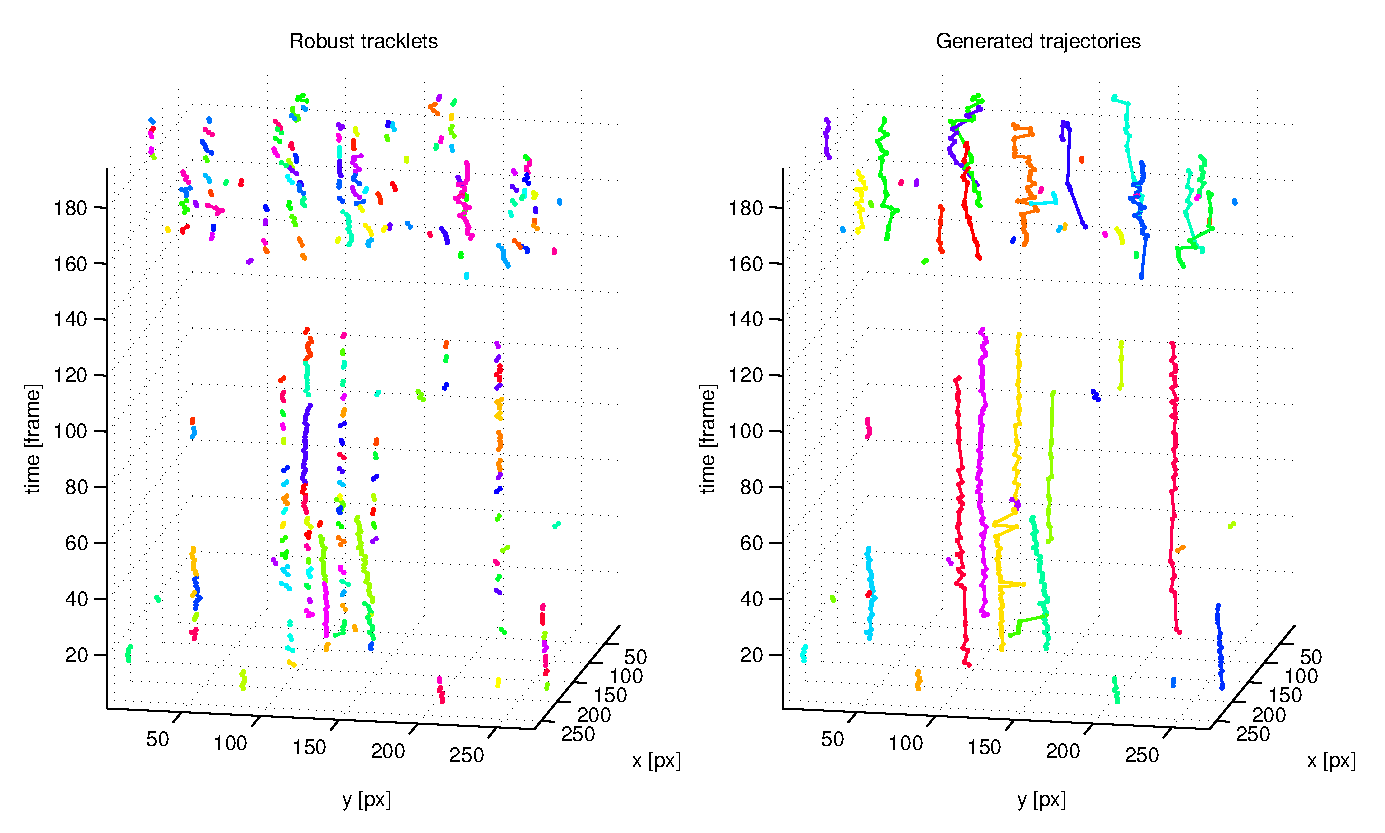
\includegraphics[width=\textwidth]{images/fig_results_tracking_analysis5}
			\caption{The tracker was able to close gaps up to length 20 in the dataset E and connect a large number of robust tracklets into coherent trajectories.}
			\label{fig:results_tracking_analysisE}
		\end{figure}

		All four dataset exceeded target effectiveness of 90. Dataset B achieved track purity of 99.7, dataset C of 87.7, dataset D of 77.2 and dataset E of 92.5. The lower track purity in dataset D can be attributed to two related reasons. First, this dataset contains a significant number of motion artefacts, arguably more than the other datasets. The second and more likely reason for the low target effectiveness is that several frames had been manually deleted from this dataset. In the original dataset more than 30\% of the frames were completely unusable; no cells were clearly discernible. These frames had been simply deleted before any analysis was performed on them. The results is that the original cell trajectories are cut, and these cuts are clearly noticeable in a few places in the image sequence. Cell trajectories where the cut is clearly visible were annotated as 2 distinct trajectories. However, since the tracker wasn't aware of this deletion it linked these individual track segments, resulting in a lower track purity value. This can be clearly seen in \cref{fig:results_tracking_analysisD} which shows the most affected trajectories.
		
		\begin{figure}[h]
			\centering				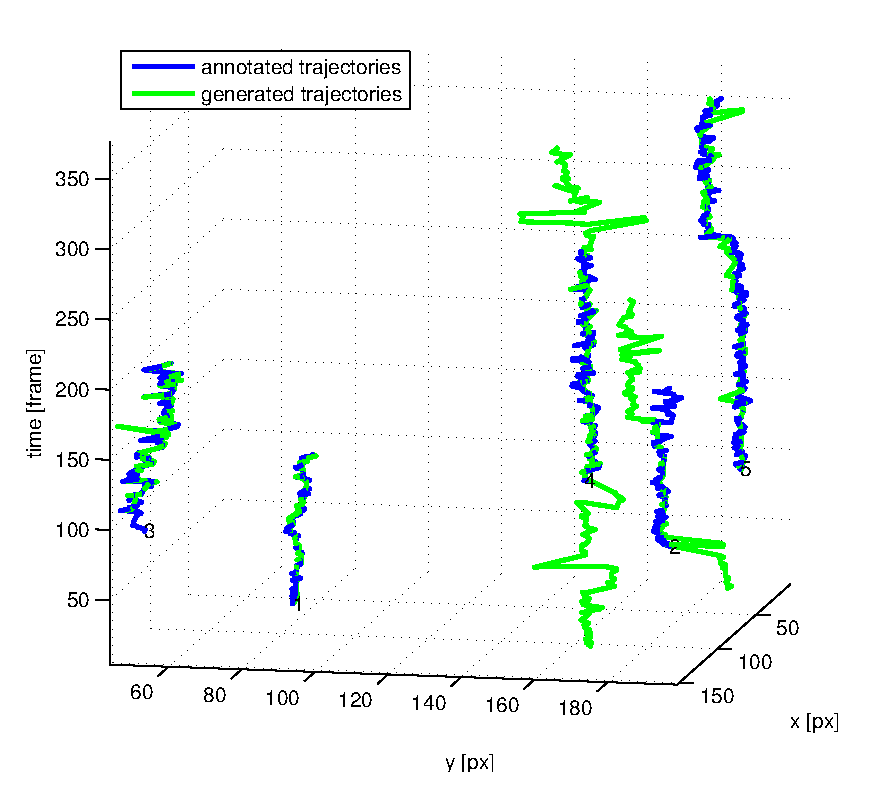
\includegraphics[width=0.6\textwidth]{images/fig_results_tracking_analysis_4}
			\caption{The tracker has linked together trajectory segments that were annotated as independent trajectories in dataset E. The sharp changes in the trajectories are due to manual deletion of a number of frames in this dataset.}
			\label{fig:results_tracking_analysisD}
		\end{figure}
		
		The comparison of ground truth annotations and \textit{detected ground truth annotations} is very high in all datasets, which tells us that the cell detector has in general detected most of cells of the evaluated trajectories (note that the position of missing detections were completed by linearly interpolating the positions of nearby detections; the high values do not mean that were almost no missed detections). The track purity for DG-DGP-P is always 100, because of the design of \textit{detected ground truth annotations} which dictates that they cannot ever be longer than the ground truth annotations.
		
		Finally, the measurements confirm the expectation that the performance of the generated trajectories relative to the \textit{detected ground truth annotations} is higher than their performance relative to ground truth annotations.
		
		The generated trajectories for each of these datasets are available in \cref{fig:results_tracker_dataset_2,fig:results_tracker_dataset_3,fig:results_tracker_dataset_4,fig:results_tracker_dataset_5} in appendix \ref{app:appendix_trackingresults}. These trajectories were obtained from trackers that were trained on all the annotated trajectories.
		
		\subsubsection{Training on a combined dataset \statusfirstdraft}
		
		The first experiment showed us the ability of the tracker to learn to correctly link trajectories from a single dataset. Often, most cells in the same dataset move in a similar mode of motion (e.g. mostly stagnant, slow translation in one direction, fast translation, frequent direction changes, etc). In this second experiment we will train the tracker on several datasets combined (at each round of the cross validation we only leave a single tracklet out of the training set for testing). We are interested in how well the tracker will be able to learn from this vast range of modes of motions, and whether it will be able to successfully track an independent cell that could exhibit any of these modes of motion. The results are shown in \cref{tab:results_tracker_combined}.
		
		\begin{table}[h]
			\centering
			\begin{tabular}{r*{3}{c}*{3}{c}}
				Dataset & \multicolumn{3}{c}{Target Effectiveness} & \multicolumn{3}{c}{Track purity} \\
				        & \textbf{GT-P} & DGT-P &     GT-DGT-P     & \textbf{GT-P} & DGT-P & GT-DGT-P \\
			\hline
				  ABCDE & \textbf{82.1} & 82.8  &       97.8       & \textbf{81.5} & 81.3  &   100    \\
				   ABCE & \textbf{81.2} & 82.9  &       96.8       & \textbf{87.4} & 87.3  &   100    \\
				    ABC & \textbf{80.7} & 83.0  &       95.8       & \textbf{88.2} & 88.2  &   100    \\
				     AB & \textbf{79.5} & 82.1  &       94.9       & \textbf{99.6} & 99.6  &   100    \\
				    BCE & \textbf{83.7} & 85.1  &       97.6       & \textbf{85.4} & 85.3  &   100
			\end{tabular} 
			\caption{Tracker performance on combined datasets.}
			\label{tab:results_tracker_combined}
		\end{table}

		A difficulty in setting up this experiments comes from the fact that the training and testing is performed on the longest tracklets of the entire dataset. Therefore, shorter image sequences are likely to be under-represented when training and testing on the dataset composed of all five datasets. Therefore the experiment was also evaluated on different combinations of combined datasets. 

		Let the combined dataset ABCDE be the basis for our analysis. This dataset achieved a target effectiveness of 82.1 and track purity of 81.5. By eliminating dataset D, which had a lower track purity when training individually, we were able to increase the track purity from 81.5 to 87.4. We peak track purity was achieved when training on the combined datasets A and B. Target effectiveness remained mostly constant in all the experiments.
		
	\subsection{Computation time \statusfirstdraft}
	
	When testing the tracker on individual datasets we also measured the time required to link all the robust tracklets into trajectories. The results are shown in \cref{tab:results_tracker_speed}. 
	
	The detection was performed on a PC with an Intel(R) Core(TM) i7-2600 CPU with a clock frequency of 3.40GHz and 8GB RAM. The MATLAB version used to measure the tracking time was 8.1.0.604 (R2013a) running in Ubuntu Linux 13.04 x64.
	
	\begin{table}[h]
		\centering
		\begin{tabular}{rrrr}
			Dataset & Total time [seconds] & Time per frame [seconds] & Number of frames per second \\
		\hline
			      B &                 2.64 &                   0.038 &                     26.5 \\
			      C &                 9.79 &                   0.078 &                     12.9 \\
			      D &                19.25 &                   0.050 &                     19.6 \\
			      E &                 5.78 &                   0.030 &                     33.6
		\end{tabular} 
		\caption{Total computation time, time per frame, and number of frames tracked per second for each dataset.}
		\label{tab:results_tracker_speed}
	\end{table}
	
	The average time per frame over all the datasets is 0.049 seconds, which is equivalent to processing 23.1 frames per second. This short computation time is negligible next to the time taken by the cell detection module. The short tracking computation permits the adjustment of the parameters $\pi_{init}$, $\pi_{term}$, $\pi_{link}$ and $\pi_{FP}$ and the regeneration the trajectories in just a few seconds.
	
	The slowest part of the cell tracking module is the computation of spatio-temporal features, especially the unoptimized code that computes the Gaussian broadening features (see \cref{sec:gaussianbroadening}).
	
\section{Limitations and areas of improvement \statusfirstdraft}
	\label{sec:results_limitations}
	
	Testing the tracker on the studied datasets has given good results as seen in \cref{fig:tracking_results_datasetBlongerthan10} which compares the annotated with the generated trajectories in dataset B.
	
	\begin{figure}[h]
		\centering
		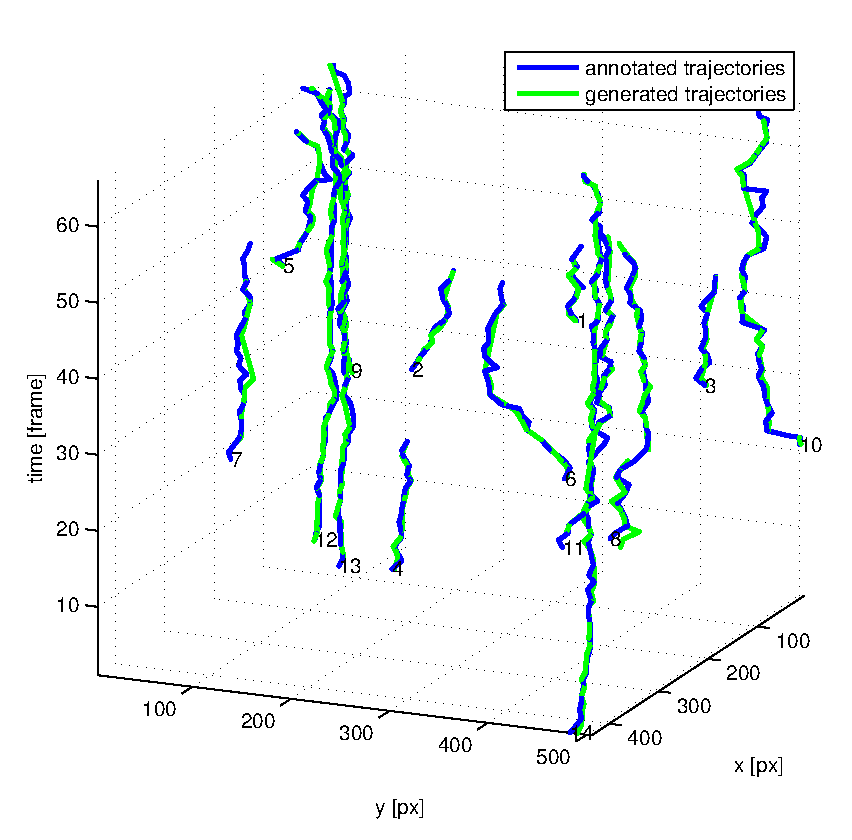
\includegraphics[width=0.7\textwidth]{images/fig_results_tracking_analysis_2}
		\caption{Comparison of annotated and generated trajectories in dataset B.}
		\label{fig:tracking_results_datasetBlongerthan10}
	\end{figure}
	
	As we have shown in \cref{fig:results_tracking_analysisE} it is also able to efficiently close very large gaps. The tracker attempts to close gaps up to the maximum length it is trained to do. Since a classifier is used to determine whether two tracklets should be linked, in general equal linking likelihoods could be computed for tracklets that are e.g. 2 frames apart than tracks that are 7 frames apart. It is possible to train the tracker to close very large gaps, e.g. more than 30 frames, but then some wrong connections are likely to occur. For example, if a cell trajectory is composed of three segments (robust tracklets) where the middle one is of length less than 30, the tracker might decide to link the first and third segments of the trajectory, making the middle segment a false positive or a short tracklet, which would be wrong. To work around this problem the closing of gaps can be performed iteratively, e.g. first for gaps of length 10, then 20 and then 30. This solution works fine, but can still introduce some smaller errors. An alternative implementation of the system could use a regression model instead of a classifier such that small caps are given a larger precedence over long gaps. However, this method requires to identify a suitable way to score the hypothesis.
	
	The tracker is able to deal with some limited jiggling of frames. However, as we have seen in \cref{fig:results_tracking_analysisD} excessive jiggling (in this case cause by the manual deletion of several frames) can results in lower performance. This issue could be resolved with a pre-processing step that would stabilize the images based on the background information present in them before inserting them to the cell tracker.
	
	Finally, let's point out that the tests performed on the tracker only measured the performance of the longest trajectories. The reason for this is to that careful annotation and review of all the trajectories in the datasets would be too time consuming and would likely include some not-insignificant amount of incorrectly linked cells.
	
	Finally, the tracker can sometimes link two independent trajectories that are close together incorrectly, as seen \cref{fig:results_tracking_analysisE}. This could be solved by computing more advanced spatio-temporal features or with a post-processing step that would detect these outliers and correct them.
	
\section{Summary \statusfirstdraft}
	\label{sec:results_summary}
	
	In this chapter we have demonstrated the performance of the cell detection and tracking modules. Several experiments on individual and combined datasets were performed to measure how well the algorithms are able to generalize to new independent datasets.
	
	The cell detector module was able to correctly detect a most of the cells in the input images in all but one dataset. The cell tracker module was then able to use these detection results to generated cell trajectories with good results. The limitations and good points of the tracker are also described and demonstrated.

	Additionally, we have measure the computation time of both the detector and tracker. We have shown that our system is able to process on average 53 frames per minute (96\% of the time spent by the cell detector). Most of the time is spend in the extraction of extremal regions and feature computation of the detection module. A considerably smaller amount of time is spent in the cell tracker module, mostly in the unoptimized spatio-temporal feature computation.